\documentclass[10pt, landscape]{article}
\usepackage[scaled=0.92]{helvet}
\usepackage{calc}
\usepackage{multicol}
\usepackage[a4paper,margin=3mm,landscape]{geometry}
\usepackage{amsmath,amsthm,amsfonts,amssymb}
\usepackage{bm}
\usepackage{color,graphicx,overpic}
\usepackage{hyperref}
\usepackage{newtxtext} 
\usepackage{enumitem}
\usepackage[table]{xcolor}
\usepackage{mathtools}
\setlist{nosep}
% for including images
\graphicspath{ {./images/} }

\pdfinfo{
  /Title (ST2132.pdf)
  /Creator (TeX)
  /Producer (pdfTeX 1.40.0)
  /Author (Jovyn Tan)
  /Subject (ST2132)
/Keywords (ST2132, nus,cheatsheet,pdf)}

% Turn off header and footer
\pagestyle{empty}

% redefine section commands to use less space
\makeatletter
\renewcommand{\section}{\@startsection{section}{1}{0mm}%
  {-1ex plus -.5ex minus -.2ex}%
  {0.5ex plus .2ex}%x
{\normalfont\large\bfseries}}
\renewcommand{\subsection}{\@startsection{subsection}{2}{0mm}%
  {-1explus -.5ex minus -.2ex}%
  {0.5ex plus .2ex}%
{\normalfont\normalsize\bfseries}}
\renewcommand{\subsubsection}{\@startsection{subsubsection}{3}{0mm}%
  {-1ex plus -.5ex minus -.2ex}%
  {1ex plus .2ex}%
{\normalfont\small\bfseries}}%
\makeatother

\renewcommand{\familydefault}{\sfdefault}
\renewcommand\rmdefault{\sfdefault}
%  makes nested numbering (e.g. 1.1.1, 1.1.2, etc)
\renewcommand{\labelenumii}{\theenumii}
\renewcommand{\theenumii}{\theenumi.\arabic{enumii}.}
\renewcommand\labelitemii{•}
\renewcommand\labelitemiii{•}

\definecolor{mathblue}{cmyk}{1,.72,0,.38}
\everymath\expandafter{\the\everymath \color{mathblue}}

% Don't print section numbers
\setcounter{secnumdepth}{0}

\setlength{\parindent}{0pt}
\setlength{\parskip}{0pt plus 0.5ex}
%% adjust spacing for all itemize/enumerate
\setlength{\leftmargini}{0.5cm}
\setlength{\leftmarginii}{0.5cm}
\setlist[itemize,1]{leftmargin=2mm,labelindent=1mm,labelsep=1mm}
\setlist[itemize,2]{leftmargin=4mm,labelindent=1mm,labelsep=1mm}

\newcommand{\cov}{\mathop{\mathrm{cov}}}
\newcommand{\var}{\mathop{\mathrm{var}}}
\newcommand{\xbar}{\bar{x}}
\newcommand{\Xbar}{\bar{X}}
\newcommand{\seq}[2][n]{#2_1, \dots, #2_{#1}}

\DeclareRobustCommand{\svdots}{% s for `scaling'
  \vbox{%
    \baselineskip=0.33333\normalbaselineskip
    \lineskiplimit=0pt
    \hbox{.}\hbox{.}\hbox{.}%
    \kern-0.2\baselineskip
  }%
}

% adding my commands
% tightcenter
\newenvironment{tightcenter}{%
  \setlength\topsep{0pt}
  \setlength\parskip{0pt}
  \begin{center}
    }{%
  \end{center}
}

% boxed
\newenvironment{tightbox}{%
  \setlength\topsep{0pt}
  \setlength\parskip{0pt}
  \begin{center}
    \begin{tabular}{|@{\hspace{\dimexpr\fboxsep+0.5\arrayrulewidth}}c@{\hspace{\dimexpr\fboxsep+0.5\arrayrulewidth}}|}
      \hline
    }
    {%
    \\ \hline
    \end{tabular}
  \end{center}
}

% fixed width box
\newenvironment{fixedbox}[1][0.7]{
  \setlength\topsep{0pt}
  \setlength\parskip{0pt}
  \begin{center}
    \begin{tabular}{|>{\centering\arraybackslash}m{#1\linewidth}|}
    \hline
  }{
  \\ \hline
  \end{tabular}
  \end{center}
}

% definition of a new term
\usepackage{soul}
\definecolor{paleyellow}{RGB}{251,243,218}
\newcommand{\definition}[2][]{\sethlcolor{paleyellow}\hl{\textbf{#2}} #1  $\rightarrow$}

% important note (attention)
\newcommand{\attention}{{\color{red}\textbf{! }}}


%  convenient absolute value symbol
\newcommand{\abs}[1]{\vert #1 \vert}

%  convenient floor and ceiling
\newcommand{\floor}[1]{\lfloor #1 \rfloor}
\newcommand{\ceil}[1]{\lceil #1 \rceil}

%  modulo with nicer spacing
\newcommand{\Mod}[1]{\ \mathrm{mod}\ #1}

%  convenient dx with nicer spacing
\newcommand{\dx}{\mathop{dx}}



% -----------------------------------------------------------------------

\begin{document}
\raggedright
\footnotesize
\begin{multicols*}{4}
  % multicol parameters
  \setlength{\columnseprule}{0.25pt}

  \begin{center}
    \fbox{%
      \parbox{0.8\linewidth}{\centering \textcolor{black}{
          {\Large\textbf{ST2132}}
        \\ \normalsize{AY23/24 SEM 1}}
        \\ {\footnotesize \textcolor{gray}{github/jovyntls}}
      }%
    }
  \end{center}

  \renewcommand{\fbox}[2][0.9\linewidth]{\begin{tightcenter}
      \fcolorbox{red}{white}{\parbox{#1}{\color{black}#2}}
    \end{tightcenter}}

  \newcommand{\fboxblue}[2][0.9\linewidth]{\begin{tightcenter}
      \fcolorbox{blue}{white}{\parbox{#1}{\color{black}#2}}
    \end{tightcenter}}


  \section{01. PROBABILITY}

  \subsection{Expectation}

  \begin{tightcenter}
    \begin{multicols*}{2}
      \textbf{discrete}: (mass) \\* \( {\displaystyle{ E(X) := \sum^n_{i=1}x_ip_i }} \) 

      \textbf{continuous}: (density) \\* \( {\displaystyle{ E(X) := \int^\infty_{-\infty} xf(x) \dx }} \) 
    \end{multicols*}
  \end{tightcenter}

  \subsubsection{expectation of a function $h(X)$}

  $ E\{h(X)\} = \begin{cases}
    \sum^n_{i=1} h(x_i)p_i &\text{$X$ is discrete} \\ 
    \int^\infty_{-\infty} h(x)f(x)\dx &\text{$X$ is continuous} \\ 
  \end{cases}$ 

  \subsection{Variance}

  \fbox{
    \begin{tightcenter} 
      \vspace{-\baselineskip}\begin{align*}
        \textbf{variance}, 
        \var(X) &:= E\{(X-\mu)^2\} \\
                &= E(X^2) - E(X)^2
      \end{align*}

      \textbf{standard deviation}, $SD(X) := \sqrt{\var(X)}$
    \end{tightcenter}
  }

  \subsubsection{useful cases}

  \begin{itemize}
    \item $E\{ X(X-\mu) \} = E(X^2) - \mu^2$
    \item $\var(X-c) = \var(X)$
    \item variance of sum = sum of variances
      $ \var(\sum^n_{i=1} X_i) = \sum^n_{i=1} \var(x_i) $ 
  \end{itemize}

  \subsection{Law of Large Numbers}

  \fbox{
    \textbf{LLN:} for a function $h$, as realisations $r \to \infty$, 

    \begin{tightcenter}
      \( {\displaystyle{ \frac{1}{r} \sum^r_{i=1}h(x_i) \to E\{h(X)\}  }} \) 

      $\xbar \to E(X)$, $\quad v \to \var(X)$
    \end{tightcenter}
  }

  \subsubsection{Monte Carlo approximation}

  simulate $\seq[r]{x}$ from $X$. by LLN, as $r \to \infty$, the approximation becomes exact

  \fbox{
    \begin{tightcenter} 
      \( {\displaystyle{ E\{h(X)\} \approx \frac{1}{r} \sum^r_{i=1} h(x_i) }} \) 
    \end{tightcenter} 
  }

  \subsection{Joint Distribution}

  (\textbf{discrete}) mass function:
  \begin{tightcenter}
    \( {\displaystyle{P( X = x_i, Y = y_j ) = p_{ij}}} \)  
  \end{tightcenter}

  (\textbf{continuous}) density function:
  \begin{tightcenter}
    \( {\displaystyle{f : \mathbb{R}^2  \to [0, \infty), \int^\infty_{-\infty} f(x, y) \dx \dy = 1}} \) 
  \end{tightcenter}

  (\textbf{expectation}) for $h : \mathbb{R}^2 \to \mathbb{R}$,
  \fbox{\begin{tightcenter} 
      \( {\displaystyle{ E\{ h(X,Y)\} = }} \) 
      \( {\displaystyle{ 
          \begin{cases}
            \sum^I_{i=1}\sum^J_{j=1} h(x_i, y_j) p_{ij} & X \text{ is discrete}
            \\ \int^\infty_{-\infty}\int^\infty_{-\infty} h(x, y) f(x, y) \dx \dy & Y \text{ is continuous}
          \end{cases}
      }} \) 
  \end{tightcenter} }

  \subsection{Covariance}

  let $\mu_X = E(X)$, $\mu_Y=E(Y)$.

  \fbox{
    \begin{tightcenter}
      \textbf{covariance}
      \begin{align*}
        \cov(X,Y) &= E\{ (X-\mu_X)(Y-\mu_Y) \}
               \\ &= E(XY) - \mu_X\mu_Y
               \\ &= \cov(Y,X)
        \\ \cov(W, aX+bY+c) &= a\cov(W, X) + b\cov(W, Y)
      \end{align*}

      \textbf{variance}

      $\var(X) = \cov(X,X)$

      \( {\scriptstyle{ \var(\sum^N_{i=1}a_iX_i) = }} \) 
      \( {\scriptstyle{  \sum^N_{i=1}a_i^2\var(X_i) + 2\sum_{1 \leq i < j \leq N} a_ia_j \cov(X_i,X_j) }} \) 
    \end{tightcenter}
  }

  \subsection{joint $=$ marginal $\times$ conditional distributions}

  \fbox{
    \begin{align*}
      f(x, y) &= f_X(x)f_Y(y \vert x) 
           \\ &= f_Y(y) f_X(x \vert y),  \quad x, y \in \mathbb{R}
    \end{align*}
  }

  \begin{itemize}
    \item $f(x, y)$ is the \textit{joint density}
    \item $f_X(x), f_Y(y)$ are the \textit{marginal densities}
    \item $f_X(\cdot \vert y)$ is the \textbf{conditional} density of $X$ given $Y=y$ 
    \item for discrete case, \textit{density} $\equiv$ \textit{probability}, $x \equiv x_i$, $y \equiv y_j$
  \end{itemize}


  \subsection{Independence}

  \fbox{
    \begin{itemize}
      \item $X, Y$ are independent $\iff \forall x, y \in \mathbb{R}$, 

        \begin{enumerate}
          \item $f(x, y) = f_X(x)f_Y(y)$ 
          \item $f_Y(y\vert x) = f_Y(y)$
          \item $f_X(x\vert y) = f_Y(x)$
        \end{enumerate}

      \item $X, Y$ are independent  $\Rightarrow$
        \begin{itemize}
          \item $E(XY) = E(X)E(Y)$ 
          \item $\cov(X,Y) = 0$
        \end{itemize}
        (the converse does not hold)
    \end{itemize}
  }

  \subsection{Conditional expectation}

  \subsubsection{discrete case}

  let $f_Y(\cdot \vert x_i)$ be the conditional pmf of $Y$ given $X = x_i$.

  \begin{tightcenter}
    \( {\displaystyle{ E[Y \vert x_i] := \sum^J_{j=1} y_j f_Y (y_j \vert x_i) }} \) 

    \( {\displaystyle{ \var[Y\vert x_i] := \sum^J_{j=1} (y_j - E[Y\vert x_i])^2 f_Y (y_j \vert x_i) }} \) 
  \end{tightcenter}

  $E[Y\vert x_i]$ is like $E(Y)$, with conditional distribution replacing marginal distribution  $f_Y(\cdot)$. 
  likewise, $\var[Y\vert x_i]$ like $\var(Y)$.

  \subsubsection{continuous case}

  \begin{tightcenter}
    \( {\displaystyle{ E[Y \vert x] := \int^\infty_{-\infty} y f_Y (y \vert x) \dy }} \) 
  \end{tightcenter}

  \begin{align*}
    \var[Y\vert x] &:= \int^\infty_{-\infty} (y - E[Y\vert x])^2 f_Y (y \vert x) \dy 
                \\ &= E(Y^2 \vert x) - \{E(Y \vert x)\}^2
  \end{align*}

  \subsection{Distributions}

  if $X$ is iid with expectation $\mu$, SD $\sigma$ and $S_n = \sum^n_{i=1}X_i$,

  \begin{tightcenter}
    \scriptsize
    \fcolorbox{red}{white}{\parbox{0.99\linewidth}{\begin{tightcenter}\color{black}
          \begin{tabular}{c|c|p{2.6cm}}
            \textbf{distribution} of $X$ & $E(X)$ & $\var(X)$ \\\hline
            $Bernoulli(p)$ & $p$ & $p(1-p)$ \\
            $Binomial(n,p)$ & $np$ & $np(1-p)$ \\
            $Geometric(n,p)$ & $1/p$ & $(1-p)/p^2$ \\
            $Multinomial(n, \mathbf{p})$ 
                             & \tiny $\left[\begin{smallmatrix}np_1 \\ np_2 \\ \svdots \\ np_k\end{smallmatrix}\right]$ 
                             & \tiny $\var(X_i) = np_i (1-p_i)$

                             $\var(X)=$ \textit{covariance matrix} $M$ \\
                             & & \scriptsize with $m_{ij} = \begin{cases}
                               \var(X_i) & \text{if }i=j
                               \\ \cov(X_i, X_j) & \text{if }i \neq j
                             \end{cases} $

          \end{tabular}
    \end{tightcenter}}}
  \end{tightcenter}

  \begin{itemize}
    \item binomial: $n$ coin flips (bernoulli) with probability $p$
      \begin{itemize}
        \item $X \sim Bin(n, p) \quad \Rightarrow$ 
          $X_i \mathop{\sim}\limits^{i.i.d.} Bernoulli(p)$
        \item $P(X=k) = \binom{n}{k} p^k (1-p)^{n-k}$
        \item $\cov(X,n-X) = -\var(X)$
      \end{itemize}
    \item multinomial: tally of $k$ possible outcomes ($n$ events)
      \begin{itemize}
        \item $\cov(X_i, X_j) < 0$
        \item $X_i \sim Bin(n, p_i)$
        \item $X_i + X_j \sim Bin(n, p_i + p_j)$
      \end{itemize}
  \end{itemize}


  \section{02. PROBABILITY (2)}

  \subsection{Mean Square Error (MSE)}

  \fcolorbox{red}{white}{\parbox{0.94\linewidth}{\begin{tightcenter}\color{black}
        \vspace{-\baselineskip}
        \begin{align*}
          MSE &= E\{ (Y-c)^2 \} \\
              &= \var(Y) + \{ E(Y) - c\}^2
        \end{align*}

        $\min MSE=\var(Y)$ when $c = E(Y)$

        if $Y$ and $X$ are correlated: 
        $MSE = \var[Y \vert x] + \{ E[Y\vert x] - c \}^2$
  \end{tightcenter}}}

  \subsubsection{mean MSE}

  $$\frac{1}{n} \sum^n_{i=1}\var[Y \vert x_i] \approx E\{ \var[Y \vert X] \}$$

  \subsubsection{random conditional expectations}

  \begin{itemize}
    \item $E[Y \vert X]$ is a r.v. which takes value $E[Y \vert x]$ with probability/density $f_X(x)$
    \item $\var[Y \vert X]$ is a r.v. which takes value $\var[Y \vert x]$ with probability/density $f_X(x)$ 
  \end{itemize}

  \fboxblue{
    $E(E[X_2 \vert X_1]) = E(X_2)$

    $\var(E[X_2 \vert X_1]) + E(\var[X_2 \vert X_1]) = \var(X_2)$
  }

  \subsection{CDF (cumulative distribution function)}

  for r.v. $X$, let $F(x) = P(X \leq x)$

  \begin{itemize}
    \item domain: $\mathbb{R}$; $\;$ codomain: $[0,1]$
  \end{itemize}

  \begin{tightcenter}
    $F(x) = \int^\infty_{-\infty} f(x) \dx$
  \end{tightcenter}

  \subsection{Standard Normal Distribution}

  \begin{tightcenter}
    $Z \sim N(0, 1)$ has density function \\* 
    \( {\displaystyle{ \phi(z) = \frac{1}{\sqrt{2\pi}} \exp \{ -\frac{z^2}{2} \}, \quad -\infty < z < \infty }} \) 
  \end{tightcenter}

  $$E(Z) = 0, \quad \var(Z) = 1$$

  \begin{tightcenter}
    \textbf{CDF}, $\Phi(x) = P(Z \leq x) = \int^x_{-\infty} \phi(z) \mathop{dz}$
  \end{tightcenter}

  \begin{itemize}
    \item  $E(Z^2) = 1$
  \end{itemize}

  \subsubsection{general normal distribution}

  \begin{tightcenter}
    \textbf{standardisation:} $\frac{X - \mu}{\sigma} \sim N(0, 1)$
  \end{tightcenter}

  \begin{itemize}
    \item for $W = a + bX$, 
      \begin{itemize}
        \item density,  $f_W(w) = \frac{d}{dw} F_W(w)$
        \item CDF, $\;\;\; F_W(w) = P(X \leq \frac{w-a}{b}) = \Phi(\frac{w-a}{b})$
      \end{itemize}
  \end{itemize}

  \subsection{Central Limit Theorem}

  \fbox{\begin{tightcenter}
      \textbf{CLT} 
      \\* as $n \to \infty$, the distribution of the standardised $S_n = \frac{S_n - n\mu}{\sqrt{n}\sigma}$ converges to $N(0,1)$

      for large $n$, approximately $S_n \sim N(n\mu, n\sigma^2)$
  \end{tightcenter}}

  \subsection{Distributions}

  \subsubsection{chi-square ($\chi^2$)}

  let $Z \sim N(0,1)$. 
  $\quad\Rightarrow$ then $Z^2 \sim \chi^2_1$ (1 degree of freedom)

  \begin{itemize}
    \item degrees of freedom = number of RVs in the sum
  \end{itemize}

  \begin{tightcenter}
    $E(Z^2) = 1, \quad E(Z^4) = 3$
    \\* $\var(Z^2) = E(Z^4) - \{ E(Z^2) \}^2 = 2$
  \end{tightcenter}

  \fbox{
    let $\seq{V} \mathop{\sim}\limits^{i.i.d.} \chi^2_1$ and $V = \sum^n_{i=1}V_i$. then 
    \begin{tightcenter}
      $V \sim \chi^2_n$

      $E(V) = n \quad \var(V) = 2n$
    \end{tightcenter}
  }

  \subsubsection{gamma}

  \fboxblue{\begin{tightcenter}
      let shape parameter $\alpha>0$, rate parameter $\lambda>0$.
      \\* The $Gamma(\alpha, \lambda)$ density is 
      \\* \( {\displaystyle{ \frac{\lambda^\alpha}{\Gamma(\alpha)} x^{\alpha-1} e^{-\lambda x}, \quad x > 0 }} \) 
      \\* $\Gamma(\alpha)$ is a number that makes density integrate to 1
  \end{tightcenter}}
  \fboxblue[0.8\linewidth]{\begin{tightcenter}
      $E(X) = \frac{\alpha}{\lambda}, \quad \var(X) = \frac{\alpha}{\lambda^2}$

      $\Gamma(\alpha +_ 1) = \alpha \Gamma (\alpha)$
  \end{tightcenter}}

  \begin{itemize}
    \item if $X_1 \sim Gamma(\alpha_1, \lambda)$ and $X_2 \sim Gamma(\alpha_2, \lambda)$ are independent, then $X_1 + X_2 \sim Gamma(\alpha_1 + \alpha_2, \lambda)$
  \end{itemize}

  \subsubsection{t distribution}

  let $Z \sim N(0, 1)$ and $V \sim \chi^2_n$ be independent. 

  \fbox{
    \begin{tightcenter}
      $\frac{Z}{\sqrt{V/n}} \sim t_n $
      \\* has a $t$ distribution with $n$ degrees of freedom.
    \end{tightcenter}
  }

  \begin{itemize}
    \item $t$ distribution is symmetric around 0
    \item $t_n \to Z \;$ as $\; n \to \infty$ (because $\frac{V}{n} \to 1$)
  \end{itemize}

  \subsubsection{\textit{F} distribution}

  \fbox{
    let $V \sim \chi^2_m$ and $W \sim \chi^2_n$ be independent. 

    \begin{tightcenter}
      $\frac{V/m}{W/n} \sim F_{m,n}$ 
      \\* has an $F$ distribution with $(m,n)$ degrees of freedom.
    \end{tightcenter}
  }

  \begin{itemize}
    \item even if $m=n$, still two RVs $V,W$ as they are independent
  \end{itemize}

  \subsection{IID Random Variables}

  let $\seq{X}$ be iid RVs with mean $\bar{X}$. 

  \fboxblue{\begin{tightcenter}
      \textbf{sample variance}, \( {\displaystyle{ S^2 = \frac{1}{n-1} \sum^n_{i=1} (X_i - \bar{X})^2 }} \) 

      $E(S^2) = \sigma^2 \quad$
      but $\quad E(S) < \sigma$
  \end{tightcenter}}

  more distributions:
  \begin{tightcenter}
    \begin{tabular}{cc}
      \fcolorbox{blue}{white}{\parbox{0.45\linewidth}{\begin{tightcenter}\color{black}
            $\frac{(n-1)S^2}{\sigma^2} \sim \chi^2_{n-1}$

            $\bar{X}$ and $S^2$ are independent
      \end{tightcenter}}}
      &
      \fcolorbox{red}{white}{\parbox{0.38\linewidth}{\begin{tightcenter}\color{black}
            $\frac{\bar{X} - \mu}{\sigma/\sqrt{n}} \sim N(0,1)$

            $\frac{\bar{X} - \mu}{S/\sqrt{n}} \sim t_{n-1}$
      \end{tightcenter}}}
    \end{tabular}
  \end{tightcenter}

  \subsection{Multivariate Normal Distribution}

  let $\bm{\mu}$ be a $k \times 1$ vector and $\bm{\Sigma}$ be a \textit{positive-definite} symmetric $k \times k$ matrix.

  \fbox{\begin{tightcenter}
      the random vector $\bm{X} = (\seq[k]{X})'$ has a 

      multivariate normal distribution $N(\bm{\mu}, \bm{\Sigma})$

      $E(\bm{X}) = \bm{\mu}, \quad \var(\bm{X}) = \bm{\Sigma}$
  \end{tightcenter}}

  \begin{itemize}
    \item two multinomial normal random vectors $\bm{X}_1$ and $\bm{X}_2$, sizes $h$ and $k$, are independent if $\cov (\bm{X}_1, \bm{X}_2) = \bm{0}_{h \times k}$
  \end{itemize}

  \section{03. POINT ESTIMATION}

  \fbox{
    for a variable $v$ in population $N$, 
    \begin{tightcenter}
      \( {\displaystyle{ 
          \mu = \frac{1}{N} \sum^N_{i=1} v_i
          \quad \quad 
          \sigma^2 = \frac{1}{N} \sum^N_{i=1} (v_i - \mu)^2
      }} \) 
    \end{tightcenter}
  }

  \begin{itemize}
    \item $\mu, \;\sigma^2$ are \ildefinition{parameters} (unknown constants)
  \end{itemize}

  \subsubsection{draws with replacement}

  \begin{tightcenter}
    random sample mean, \( {\displaystyle{ \Xbar = \frac{1}{n}\sum^n_{i=1}X_i }} \) 

    $E(\Xbar) = \mu$, $\var(\Xbar) = \frac{\sigma^2}{n}$

    $E(X_i) = \mu$, $\qquad \var(X_i) = \sigma^2$
  \end{tightcenter}

  \begin{itemize}
    \item same distribution: $x_i$, $X_i$, population distribution 
    \item the error in $\xbar$ is $\mu - \xbar$; $\quad$ it cannot be estimated
  \end{itemize}

  \subsubsection{representativeness}

  \begin{itemize}
    \item $\seq{X}$ is \textbf{representative} of the population
      \begin{itemize}
        \item as $n$ gets larger, $\Xbar$ gets closer to $\mu$
      \end{itemize}
    \item $\seq{x}$ are \textit{likely} representative of the population
  \end{itemize}

  \subsection{Point estimation of mean}

  a population (size $N$) has unknown mean $\mu$, variance $\sigma^2$.

  \subsubsection{standard error}

  \fbox{\begin{tightcenter}
      SE is a constant by definition:

      $SE = SD(\hat{X}) = \frac{\sigma}{\sqrt{n}}$

      point estimation of mean: SE ($\xbar$) is estimated as $\frac{s}{\sqrt n}$
  \end{tightcenter} }

  \subsection{Simple random sampling (SRS)}

  $n$ random draws \textit{without replacement} from a population

  \fbox{
    \begin{tightcenter}
      for $i \neq j$, $\cov(X_i, X_j) = -\frac{\sigma^2}{N-1}$
    \end{tightcenter}
  }

  \fbox{
    \begin{itemize}
      \item if $n/N$ is relatively large, account for $\cov(X_i, X_j)$
        \( {\displaystyle{ \qquad E(\Xbar) = \mu, \quad \var(\Xbar) = \frac{N-n}{N-1}\frac{\sigma^2}{n} }} \) 
      \item if $n << N$, then SRS is like sampling \textit{with replacement}
        (treat the data as IID RVs $\seq{X}$)
        $$E(\Xbar) = \mu, \quad \var(\Xbar) = \frac{\sigma^2}{n}$$
    \end{itemize}
  }

  \subsubsection{estimating proportion $p$}

  \begin{itemize}
    \item the estimate of $\sigma$ is $\hat{\sigma}$, not $s$
    \item unbiased estimator $\hat p$
      \begin{itemize}
        \item $E(\hat p) = p, \quad \var(\hat p) = \frac{p(1-p)}{n}, \quad SE = SD(\hat p)$
      \end{itemize}
  \end{itemize}

  \section{04. ESTIMATION (SE, bias, MSE)}

  for random draws $\seq{X}$ \textit{with replacement}

  \subsection{MSE and bias}

  suppose measurements were from a population with mean $w + b$ where
  $b$ is a constant:
  $\quad x_i = w + b + \epsilon_i$
  \begin{itemize}
    \item $E(\Xbar) = w + b$, $\quad SD(\Xbar) = \frac{\sigma}{\sqrt n}$
      \begin{itemize}
        \item $SE = \frac{\sigma}{\sqrt n}$ measures how far $\xbar$ is from $w+b$, not $w$
      \end{itemize}
    \item if $b\neq 0$, then $\xbar$ is a biased estimate for $w$
    \item $MSE = E\{(\Xbar - w)^2\} = \frac{\sigma^2}{n} + b^2$
  \end{itemize}

  \subsubsection{general case}

  \fboxblue{\begin{tightcenter}
      let $\theta$ be a parameter and $\hat \theta$ be an estimator (RV).

      $SE = SD(\hat\theta)$, $\quad$ bias = $E(\hat\theta) - \theta$,

      $MSE = E\{(\hat\theta - \theta)^2\} = SE^2 + bias^2$

      as $n \to \infty, \; MSE \to b^2$
  \end{tightcenter} }

  \section{05. INTERVAL ESTIMATION}

  let $\seq{x}$ be realisations of IID RVs $\seq{X}$ with unknown $\mu = E(X_i)$ and $\sigma^2 = \var(X_i)$. 

  \begin{tightcenter}
    \textbf{point estimation:} $\mu \approx \xbar \pm \frac{s}{\sqrt n}$

    \textbf{interval estimation:} interval contains $\mu$ with some confidence level
  \end{tightcenter}

  interval estimation works well if
  \begin{itemize}
    \item $X_i$ has a normal distribution, for any $n > 1$ 
    \item $X_i$ has any other distribution but $n$ is large
  \end{itemize}

  \subsection{normal ''upper-tail quantile'' $z_p$}

  \fbox{\begin{tightcenter}
      let $Z \sim N(0,1)$. let $z_p$ be the $(1-p)$-quantile of $Z$.

      $p=\Pr(Z > z_p)$
  \end{tightcenter} }

  \subsubsection{(case 1) normal distribution with known $\sigma^2$}

  $\seq{X} \mathop{\sim}\limits^{i.i.d.} N(0,1)$ with known $\sigma^2$.

  for $0<\alpha<1$, $\;\Pr(-z_{\frac{\alpha}{2}} \leq Z \leq z_{\frac{\alpha}{2}}) = 1-\alpha$

  \fbox{\begin{tightcenter}
      \textbf{confidence interval for $\mu$:}
      the random interval 

      \( {\displaystyle{ \left( \Xbar-z_{\frac{\alpha}{2}}\frac{\sigma}{\sqrt n}, \Xbar+z_{\frac{\alpha}{2}}\frac{\sigma}{\sqrt n} \right) }} \) 

      contains $\mu$ with probability (confidence level) $1-\alpha$
  \end{tightcenter} }

  \subsubsection{(case 2) normal distribution with unknown $\sigma^2$}

  replace $\sigma$ with $S$ and use $t$ distribution:

  \begin{tightcenter}
    for $0 < p < 1$, let $t_{p,n}$ be such that 

    $\Pr(t_n > t_{p,n}) = p$

    as $n \to \infty, \;\; t_{n,p} \to z_p$

    \fbox{\begin{tightcenter}
        the random interval

        $\left(\Xbar - t_{\frac{\alpha}{2}, n-1} \frac{S}{\sqrt n},  \Xbar + t_{\frac{\alpha}{2}, n-1} \frac{S}{\sqrt n}\right)$

        contains $\mu$ with probability $1-\alpha$.
    \end{tightcenter} }
  \end{tightcenter}

  \subsubsection{(case 3) general distribution with unknown $\sigma^2$}

  \begin{itemize}
    \item CLT: for large $n$, approximately $\frac{S_n - n\mu}{\sqrt n \sigma} \sim N(0,1)$
    \item since $\frac{S_n - n\mu}{\sqrt n \sigma} =  \frac{\Xbar - \mu}{\sigma / \sqrt n}$,
  \end{itemize}

  \fbox{\begin{tightcenter}
      for large $n$, the random interval

      \( {\displaystyle{ \left( \Xbar-z_{\frac{\alpha}{2}}\frac{S}{\sqrt n}, \Xbar+z_{\frac{\alpha}{2}}\frac{S}{\sqrt n} \right) }} \) 

      contains $\mu$ with probability $\approx 1-\alpha$
  \end{tightcenter}}

  \begin{itemize}
    \item for SRS, multiply $SE$ by correction factor $\sqrt{\frac{N-n}{N-1}}$
    \item contains $\mu$ with probability $<1-\alpha$
    \item probability $\to 1-\alpha$ as $n \to \infty$
    \item \textbf{exception}: for Bernoulli, $\sigma = \sqrt{p(1-p)}$ is not estimated by $s$, but by replacing $p$ with the sample proportion
  \end{itemize}

  \section{06. METHOD OF MOMENTS}

  modified notation of mass/density functions:

  \begin{itemize}
    \item \textbf{bernoulli}: $f(x\vert p) = p^x (1-p)^{1-x}, \quad x=0,1$
      \begin{itemize}
        \item parameter space is $(0,1)$
      \end{itemize}
    \item \textbf{poisson}: $f(x \vert \lambda) = \frac{\lambda^xe^{-\lambda}}{x!}, \quad x=0,1,\dots$
      \begin{itemize}
        \item parameter space is $\mathbb{R}_+$
      \end{itemize}
  \end{itemize}

  \subsection{parameter estimation}

  assuming data $\seq{x}$ are realisations of IID RVs $\seq{X}$ with mass/density function  $f(x \vert \theta)$, 
  where $\theta$ is unknown in parameter space $\Theta$.

  \begin{itemize}
    \item 2 methods to estimate $\theta$ :
      \begin{itemize}
        \item method of moments (MOM)
        \item method of maximum likelihood (MLE)
      \end{itemize}
    \item the estimate of $\theta$ is a realisation of an estimator $\hat \theta$ 
    \item parameter space $\Theta$: set of values that can be used to estimate the real parameter value $\theta$
      \begin{itemize}
        \item e.g. for $N(\mu, \sigma^2)$, parameter space $\Theta = \mathbb{R} \times \mathbb{R}_+$
      \end{itemize}
  \end{itemize}

  \subsection{Moments of an RV}

  \fbox{\begin{tightcenter}
      the $k$-th moment of an RV $X$ is

      $\mu_k = E(X^k)$, $\quad k = 1,2,\dots$
  \end{tightcenter}}

  \subsubsection{estimating moments}

  let $\seq{X}$ be IID with the same distribution as $X$. 

  \fbox{\begin{tightcenter}
      the $k$-th sample moment  is

      $\hat{\mu}_k = \frac{1}{n} \sum^n_{i=1}X_i^k$

      $E(\hat\mu_k) = E(\frac{1}{n}\sum^n_{i=1} x^k_i) = \mu_k$  $\quad\Rightarrow$ unbiased!
  \end{tightcenter}}

  \subsubsection{MOM: general}

  let $X \sim Distribution(\theta)$. to obtain $\xbar$ and $SE$:

  \fbox[0.95\linewidth]{
    \begin{enumerate}
      \item $\mu = \mu_1$, $\quad \sigma^2 = \mu_2 - \mu_1^2$
      \item express parameters in terms of moments
      \item estimate MOM estimator using sample mean $\xbar$: $\hat\theta = \hat\mu_1 = \Xbar$
      \item obtain $SE = SD(\hat\theta) = \sqrt{\var(\hat\theta)} = \sqrt{\frac{1}{n} \var(X)}$
    \end{enumerate}

    \begin{tightcenter}
      $\theta \approx \xbar \pm \sqrt\frac{\var(X)}{n}$
    \end{tightcenter}
  }

  \section{07. MLE}

  \subsection{Likelihood function}

  let $\seq x$ be realisations of iid rvs $\seq X$ with density $f(x \vert \theta), \; \theta \in \Theta \subset \mathbb{R}^k$.

  \fbox{\begin{tightcenter}
      \ildefinition{likelihood function} $L : \Theta \to \mathbb{R}_+$ is
      \vspace{-0.7\baselineskip}\begin{align*}
        L(\theta) 
          &= \prod^n_{i=1} f(x_i \vert \theta) 
       \\ &= f(x_1 \vert \theta) \times \dots \times f(x_n \vert \theta) 
      \end{align*}

      \ildefinition{loglikelihood function} $\ell : \Theta \to \mathbb{R}$ is

      \( {\displaystyle{ \ell(\theta) = \log L(\theta) = \sum^n_{i=1}\log f(x_n \vert \theta) }} \) 

      (can omit additive constants ($\ell$)/constant factors ($L$))
  \end{tightcenter} }

  \subsection{Maximum Likelihood Estimation (MLE)}

  \begin{itemize}
    \item \definition[of $L$]{maximiser} the maximum likelihood estimate of $\theta$ (a realisation of the MLEstimator $\hat\theta$)
      \begin{itemize}
        \item maximiser of loglikelihood $\ell = \log L$ over $\Theta$
      \end{itemize}
  \end{itemize}

  find the value of $\theta$ that maximises (log)likelihood:
  \begin{enumerate}
    \item calculate likelihood $L$, loglikelihood $\ell$
    \item differentiate loglikelihood $\ell$: $\ell'(\theta) = 0$
    \item confirm max point: $\ell''(\theta) < 0$
  \end{enumerate}

  \subsection{ML vs MOM}

  \begin{itemize}
    \item MOM estimates can always be written in terms of the data (sample moments)
      \begin{itemize}
        \item ML uses *
      \end{itemize}
    \item ML has better (smaller) SE and bias than MOM
    \item MOM/ML estimates are asymptotically unbiased 
      \begin{itemize}
        \item as $n \to \infty$, $E(\hat\theta_n) \to \theta$
      \end{itemize}
  \end{itemize}

  \subsection{Kullback-Liebler divergence (KL)}

  let $\mathbf{q} = (\seq[k]{q})$ and $\mathbf{p} = (\seq[k]{p})$ be strictly positive probability vectors.

  \fbox{
    \begin{tightcenter}
      the \ildefinition{KL divergence} between $\mathbf{q}$ and $\mathbf{p}$ is

      \( {\displaystyle{ d_{KL}(\mathbf{q}, \mathbf{p}) = \sum^k_{i=1}q_i \log (\frac{q_i}{p_i}) }} \) 
    \end{tightcenter}

    \begin{itemize}
      \item $d_{KL}(\mathbf{q}, \mathbf{p}) \geq 0$ $\quad$ 
        (equality $\iff \mathbf{q} = \mathbf{p}$)
      \item $d_{KL}(\mathbf{q}, \mathbf{p}) \neq d_{KL}(\mathbf{p}, \mathbf{q})$ 
    \end{itemize}

  } 

  \begin{itemize}
    \item used to maximise $\ell$ to find MLE for multinomial
    \item let $\mathbf{q}$ be the MOM estimate for $\mathbf{p}$. for any $\mathbf{p}$, $\ell(\mathbf{q}) - \ell(\mathbf{p}) = \sum^k_{i=1}x_i \log q_i - \sum^k_{i=1} x_i \log p_i$ 
      $\qquad\qquad\qquad = n \, d_{KL}(\mathbf{q}, \mathbf{p}) \geq 0$
      \begin{itemize}
        \item $\ell(\mathbf{q}) - \ell(\mathbf{p}) = 0 \iff \mathbf{p} = \mathbf{q} = \frac{\mathbf{x}}{n}$
      \end{itemize}
  \end{itemize}

  \subsection{Hardy-Weinberg equilibrium (HWE)}

  let $\theta$ be the proportion of $a$. 

  \fbox[0.95\linewidth]{
    \begin{tightcenter}
      the population is in \ildefinition{HWE} if 

      $f(aa) = \theta^2,\quad f(aA) = 2\theta(1-\theta),\quad f(AA) = (1-\theta)^2$
    \end{tightcenter}
  }

  \begin{itemize}
    \item (e.g. genotypes)
      Under HWE, the number of $a$ alleles in an individual has a $Binom(2, \theta)$ distribution
      \begin{itemize}
        \item for $n$ randomly chosen people, number of $a$ alleles $(AA, Aa, aa) \sim Multinomial(n, \theta)$
      \end{itemize}
  \end{itemize}

  \subsubsection{Multinomial ML estimation}

  for $(X_1, X_2, X_3) \sim Multinomial(n, \mathbf{p})$

  where $p_1 = (1-\theta)^2, \, p_2 = 2\theta(1-\theta), \, p_3 = \theta^2$

  \begin{itemize}
    \item $L(\theta) = p_1^{x_1} \, p_2^{x_2} \, p_3^{x_3}$
      $\qquad = 2^{x_2} \, (1-\theta)^{2x_1 + x_2} \, \theta^{x_2 + 2x_3}$
    \item $\ell(\theta) = x_2 \log 2 + (2x_1 + x_2) \log (1-\theta) + (x_2 + 2x_3)\log \theta$
    \item ML estimator: $\hat\theta = \frac{X_2 + 2X_3}{2n}$
    \item SE estimation: $\sqrt{\frac{\theta(1-\theta)}{2n}}$
      \begin{itemize}
        \item $X_2 + 2X_3$ is the number of $a$ alleles: $Binom(2n, \theta)$
          $\quad \Rightarrow \var(\hat\theta) = \frac{\theta(1-\theta)}{2n}$
      \end{itemize}
  \end{itemize}

  \section{08. LARGE-SAMPLE DISTRIBUTION OF MLEs}

  \subsection{asymptotic normality of ML estimator}

  let $\hat\theta_n$ be the ML estimator of $\theta \in \Theta \subset \mathbb{R}$, based on iid RVs $\seq{X}$ with density $f(x \vert \theta)$. 

  \fboxblue[0.7\linewidth]{\begin{tightcenter}
      for large $n$, approximately 

      $\hat\theta_n \sim N(\theta, \frac{\mathcal{I}(\theta)^{-1}}{n})$ 
  \end{tightcenter} } 

  \subsection{Fisher Information}

  let $X$ have density $f(x \vert \theta)$, $\theta \in \Theta \subset \mathbb{R}^k$.

  \fboxblue{\begin{tightcenter}
      the \ildefinition{Fisher information} is the $k\times k$ matrix
      $\mathcal{I}(\theta) = -E\left[ \frac{d^2\log f(X \vert \theta)}{d \theta^2} \right]$
  \end{tightcenter} } 

  \begin{itemize}
    \item $\mathcal{I}(\theta)$ is symmetric, with $(i j)$-entry $-E\left[ \frac{\delta^2\log f(X \vert \theta)}{\delta \theta_i \delta \theta_j} \right]$
    \item $\mathcal{I}(\theta)$ measures the information about $\theta$ in one sample $X$.
  \end{itemize}

  \subsection{Asymptotic normality: general}

  \begin{enumerate}
    \item obtain \textbf{fisher information}, $\mathcal{I}(\theta) = -E\left( \frac{d^2\log f(X \vert \theta)}{d \theta^2} \right)$
    \item \textbf{asymptotic normality}: for large $n$, approximately
      $\hat\theta_n \sim N(\theta, \frac{\mathcal{I}(\theta)^{-1}}{n})$ 
      $\quad$ (not necessarily exact)
  \end{enumerate}

  \subsection{Approximate CI with ML estimate}

  $\hat\theta_n$ is the ML estimator of $\theta$ based on iid RVs $\seq X$.

  \begin{itemize}
    \item for large $n$, approximately $\hat\theta_n \sim N(\theta, \frac{\mathcal{I}(\theta)^{-1}}{n})$.
    \item the random interval 
      $\left( \hat\theta_n - z_{\frac{\alpha}{2}} \sqrt \frac{\mathcal{I}(\theta)^{-1}}{n}, \hat\theta_n + z_{\frac{\alpha}{2}} \sqrt \frac{\mathcal{I}(\theta)^{-1}}{n} \right)$ 

      covers $\theta$ with probability $\approx 1-\alpha$
  \end{itemize}

  \subsection{Scope of asymptotic normality of ML estimators}

  \begin{itemize}
    \item let $\hat\theta^n$ be the ML estimator of $\theta$. 
      For strictly increasing or strictly decreasing $h : \Theta \to \mathbb{R}$, $h(\hat\theta^n)$ is the ML estimator of $h(\theta)$.
      for large $n$, $h(\hat\theta^n)$ is approximately normal
  \end{itemize}

  \subsection{population mean vs parameter}

  for $n$ random draws with replacement from a population with mean $\mu$ and variance $\sigma^2$,

  \begin{tightcenter}\begin{tabular}{r|ccc}
    Estimator & $E$ & $\var$ & Distribution \\ \hline
    {\tiny random sample mean}, $\hat\mu$ & $\mu$ & $\frac{\sigma^2}{n}$ & $\approx$ normal \\
    {\tiny ML estimator}, $\hat\theta_n$ & $\approx \theta$ & $\approx\frac{\mathcal{I}(\theta)^{-1}}{n}$ & $\approx$ normal
  \end{tabular}\end{tightcenter}

  $\hat\theta_n$ is not normal (but may approach normal for large $n$)

  \subsection{Cram\'er-Rao inequality}

  \fbox{
    \begin{tightcenter}
      if $\hat\theta_n$ is unbiased, then 
      $\var(\hat\theta_n) \geq \frac{\mathcal{I}(\theta)^{-1}}{n}$ 

      \ildefinition{efficient} $\iff$ equality
    \end{tightcenter}
  }

  % TODO this is from the quiz?
  $E( \frac{d\log f(X \vert \lambda)}{d\lambda} ) = 0$


  \section{09. HYPOTHESIS TESTING}

  let $\seq x$ be realisations of IID $N(\mu, \sigma^2)$ RVs $\seq X$ 
  where $\mu$ is a parameter and $\sigma$ is known.

  \fboxblue{
    \begin{tightcenter}
      \ildefinition{null hypothesis}, $H_0 : \mu = \mu_0$

      \ildefinition{alternative hypothesis}, $H_1 : \mu = \mu_1$
    \end{tightcenter}
  }

  if $\sigma$ is unknown or $\seq x \not\sim N(\mu,\sigma^2)$, we can use CLT

  \subsection{09.1. Rejection region}

  \begin{tightcenter}
    \textbf{one-tailed test}: $\quad H_0: \mu = \mu_0$, $\quad H_1 : \mu = \mu_1 > \mu_0$

    \textbf{two-tailed test}: $\quad H_0: \mu = \mu_0$, $\quad H_1 : \mu = \mu_1 \neq \mu_0$
  \end{tightcenter}

  \fbox[0.98\linewidth]{
    \begin{enumerate}
      \item state hypotheses $H_0, H_1$. 
      \item reject $H_0$ if $\xbar - \mu_0 > c$  (or $|\xbar - \mu_0| > c$)
      \item $c = z_{\alpha(/2)} \frac{\sigma}{\sqrt n}$ by normalising $\alpha = P_{H_0} (\Xbar > \mu_0 + c)$
        \begin{itemize}
          \item since under $H_0$, $X \sim N(\mu_0, \frac{\sigma^2}{n})$.
        \end{itemize}
      \item \textbf{rejection region}: reject $H_0$ if $\dots$
        \begin{itemize}
          \item $\xbar \in \left( \mu_0 + c, \infty \, \right)$
            \item $\xbar \in (-\infty,\; \mu_0 - c) \cup (\mu_0 + c, \infty)$
        \end{itemize}
    \end{enumerate}
  }

  \fbox{
    \begin{tightcenter}
      composite $H_1$: (does not change rejection region)

      \textbf{one-tailed test}: $\quad H_0: \mu = \mu_0$, $\quad H_1 : \mu > \mu_0$
      \textbf{two-tailed test}: $\quad H_0: \mu = \mu_0$, $\quad H_1 : \mu \neq \mu_0$
    \end{tightcenter}
  }

  \subsubsection{Size and power}

  \fbox[0.98\linewidth]{
    \begin{tightcenter}\begin{tabular}{c|cc}
      Hypothesis & $\xbar < \mu_0 + c$ & $\xbar > \mu_0 + c$ \\\hline
      $H_0$ & $\checkmark$ not reject $H_0$ & {$\color{red}\times (I)$ } reject $H_0$ \\
      $H_1$ & $\color{red}\times (II)$ not reject $H_0$ & $\checkmark$ reject $H_0$
    \end{tabular}\end{tightcenter}

    \begin{itemize}
      \item type $\color{red}I$ error: rejecting  $H_0$ when it is true
      \item type $\color{red}II$ error: not rejecting $H_0$ when it is false
    \end{itemize}
  }

  \begin{itemize}
    \item \definition[of a test]{size} (aka \ildefinition{level}) probability of a Type $I$ error
      \begin{itemize}
        \item $\alpha := P_{H_0} (\Xbar > \mu_0 + c)$
        \item (for 2-tail) corresponds to a $(1-\alpha)$-CI for $\mu$
      \end{itemize}
    \item \definition[of a test]{power} $1-$ probability of a Type $II$ error
      \begin{itemize}
        \item $\beta := P_{H_1} (\Xbar > \mu_0 + c)$ $\quad \Rightarrow \text{power} = 1-\beta$
        \item as $n \to \infty$, \ power $\to 1$
      \end{itemize}
    \item $\uparrow c : \quad \downarrow \alpha, \downarrow \beta \;$ ($\downarrow$ type $I$ error, $\uparrow$ type  $II$ error)
  \end{itemize}

  \begin{tightcenter}
    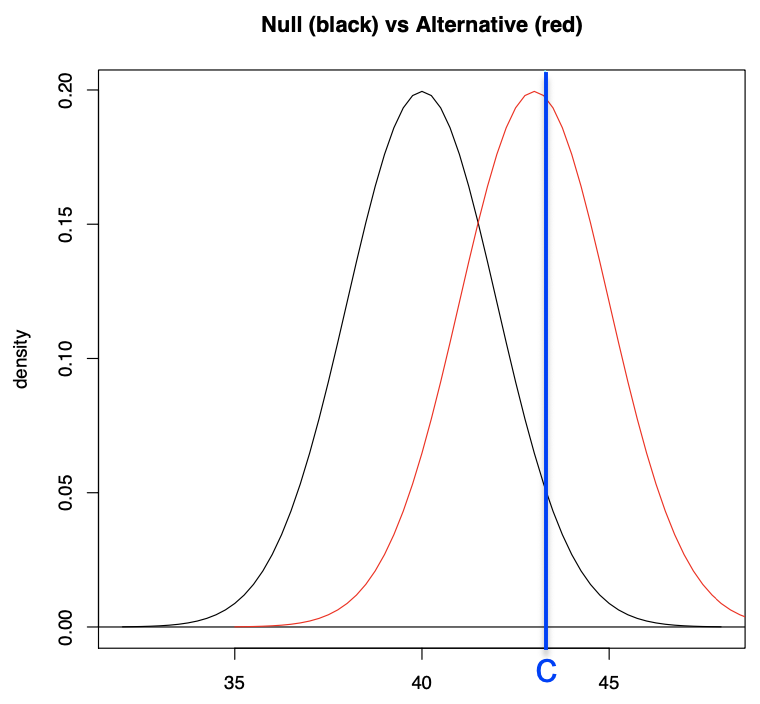
\includegraphics[width=0.65\linewidth]{st2132-hypothesis-testing-c.png} 
  \end{tightcenter}

  \subsection{09.2. $P$-value}

  \fboxblue[0.97\linewidth]{
    \begin{itemize}
      \item \definition{$P$-value} the probability under $H_0$ that the random test statistic is more extreme than the observed test statistic
        \begin{itemize}
          \item small $p$-value = more ''extreme'' (more doubt)
        \end{itemize}
    \end{itemize}
  }
  \fbox{
    \begin{itemize}
      \item reject $H_0$ at level $\alpha \iff P<\alpha$
      \item generally, $P$-value for two-tailed test is double that of one-tailed test
    \end{itemize}
  }

  \subsubsection{formulae for $P$-value}

  \fbox[0.95\linewidth]{
    $H_1 : \mu > \mu_0$ 

    $\qquad$ $P = P_{H_0} (\Xbar > \xbar) = \Pr \left( Z > \frac{\xbar - \mu_0}{\sigma / \sqrt n} \right)$

    $H_1 : \mu < \mu_0$ 

    $\qquad$ $P = P_{H_0} (\Xbar < \xbar) = \Pr \left( Z < \frac{\xbar - \mu_0}{\sigma / \sqrt n} \right)$

    $H_1 : \mu \neq \mu_0$

    $\;$ $P = P_{H_0} (| \Xbar-\mu_0 | > | \xbar-\mu_0 |) = \Pr \left( |Z| > \frac{|\xbar - \mu_0|}{\sigma / \sqrt n} \right)$
  }

  \section{10. GOODNESS-OF-FIT}

  \subsection{General LR test}

  \begin{itemize}
    \item $n$ iid RVs with density defined by $\theta \in \Omega_1$
    \item smaller model $\Omega_0$ is  \ildefinition{nested} in $\Omega_1$ ($\Omega_0 \subset \Omega_1$)
      \begin{itemize}
        \item $L_1 \geq L_0$ $\quad$ ($L_0$ is the maximum over a subset of $L_1$)
        \item larger $L_1 / L_0 \Rightarrow$ poorer fit for smaller model
      \end{itemize}
  \end{itemize}

  \fbox[0.7\linewidth]{ \begin{tightcenter}
      $H_0 : \theta \in \Omega_0 \qquad H_1 : \theta \in \Omega_1 \backslash \Omega_0$
  \end{tightcenter} }

  \fboxblue{
    \begin{tightcenter}
      \ildefinition{LR statistic} (to test $H_0$)

      $G = 2\log \left(\frac{L_1}{L_0}\right) = 2(\log L_1 - \log L_0)$

      \smallskip
      if $\theta \in \Omega_0$, as $n \to \infty$, 

      $G \sim \chi^2_{\dim\Omega_1-\dim\Omega_0}$
    \end{tightcenter}
  }

  \subsubsection{LR test}

  \fbox[0.95\linewidth]{
    \begin{enumerate}
      \item LR test statistic, 
        \\* $G = 2 \log \left( \frac{L_1}{L_0} \right) = 2( \log L_1 - \log L_0 )$
      \item null hypothesis, $H_0 :$ the tighter model holds
      \item approximate $P$-value to $\chi^2$-distribution:
        \begin{itemize}
          \item $P \approx \Pr \left( \chi^2_{deg} > G \right)$
          \item calculate $g$ using \textit{observed count} $x_i$ and \textit{expected count} (under $H_0$, calculated using ML estimate)
        \end{itemize}
      \item high $P$-value = better fit for tighter model
    \end{enumerate}
  }

  \subsection{General Multinomial LR test}

  let $(\seq[k]{X}) \sim Multinomial(n, \mathbf{p})$. 
  then $\mathbf{p} \in \Omega_1$, the set of all positive probability vectors of length $k$.

  let subspace $\Omega_0 = \left\{ (p_1(\theta), \dots, p_k(\theta)) : \theta \in \Theta \subset \mathbb{R}^h \right\}$ 
  with $\dim\Omega_0 < \dim\Omega_1 = k-1$.
  $\quad$ to test $H_0 : \mathbf{p} \in \Omega_0$

  \begin{itemize}
    \item $G = 2\sum^k_{i=1} X_i \log \left( \frac{X_i}{np_i(\hat\theta)} \right)$
      \begin{itemize}
        \item for $\Omega_1$: $\log L_1 = \sum^k_{i=1} X_i \log (\frac{X_i}{n})$
        \item for $\Omega_0$: $\log L_0 = \sum^k_{i=1} X_i \log p_i(\hat\theta)$
      \end{itemize}
    \item $P = P_{H_0} (G > g) \approx \Pr (\chi^2_{k-1-\dim\Omega_0} > g)$ for large $n$.
    \item to compute $g$, replace
      \begin{itemize}
        \item $X_i$ with \textit{observed count} $x_i$
        \item $np_i(\hat\theta)$ with \textit{expected count} (under $H_0$) using ML estimate of  $\theta$
      \end{itemize}
  \end{itemize}

  \subsection{Test of independence}

  for a population with attributes $q$ and $r$, 
  let $p_{ij} = q_i \times r_j$ be the population proportion of people with $q=q_i$ and $r=r_j$.

  \begin{itemize}
    \item let $(X_{ij}, 1 \leq i \leq I, 1 \leq j \leq J) \sim Multinomial(n, \mathbf{p})$.
      $\mathbf{p} \in \Omega_1$, where $\dim \Omega_1 = IJ - 1 = k-1$.
    \item $H_0 : $ the two categories $q,r$ are independent
      \begin{itemize}
        \item if $q,r$ are independent, then $\exists $ positive numbers $\sum^I_{i=1}q_i = \sum^J_{j=1}r_j = 1$
          such that $p_{ij} = q_i \times r_j$, $\; 1 \leq i \leq I, 1 \leq j \leq J$
      \end{itemize}
    \item under $H_0$, for large  $n$, approximately $G \sim \chi^2_{(I-1)(J-1)}$
      \begin{itemize}
        \item $\dim\Omega_0 = (I-1) + (J-1) = I+J-2$
        \item $\dim\Omega_1 - \dim\Omega_0 = (I-1)(J-1)$
      \end{itemize}
    \item $G = 2(\log L_1 - \log L_0) = 2\sum_{ij} X_{ij} \log \left( \frac{X_{ij}}{X_{i+} X_{+j}/n} \right)$ 
      \begin{itemize}
        \item $\Omega_1$ : $\log L_1 = \sum_{ij} X_{ij} \log ( \frac{X_{ij}}{n} )$
        \item $\Omega_0$ : $\scriptscriptstyle\log L_0 = \sum_i X_{i+} \log ( \frac{X_{i+}}{n} ) + \sum_{+j} X_{+j} \log ( \frac{X_{+j}}{n} )$
      \end{itemize}
    \item $P$-value $= \Pr\left(\chi^2_{(I-1)(J-1)} > g\right)$
      \begin{itemize}
        \item the data $x_{ij}$ are the \textit{observed counts}
        \item the data $x_{i+} x_{+j}/n$ are the \textit{expected counts}
      \end{itemize}
  \end{itemize}

  \subsubsection{Normal LR test}

  $\seq{X} \mathop{\sim}\limits^{i.i.d.} N(\mu, \sigma^2)$.
  to test $H_0 : \mu = 0$:

  $ \begin{array}{c|c|c|c|c}
    \sigma & \Omega_1 & \dim\Omega_1 & \Omega_0 & \dim\Omega_0 \\\hline
    \text{known} & \mathbb{R} & 1 & \{0\} & 0 \\
    \text{unknown} & \mathbb{R}\times \mathbb{R}_+ & 2 & \{0\} \times \mathbb{R}_+ & 1
  \end{array} $

  under $H_0$, for large $n$, approximately $G \sim \chi^2_1$

  \begin{itemize}
    \item \textbf{case 1}: $\sigma$ known
      \begin{itemize}
        \item $\Omega_0 : \log L_0 = -\frac{n\hat\mu^2}{2\sigma^2}$, 
          $\;\Omega_1 : \log L_1 = -\frac{n\hat\sigma^2}{2\sigma^2}$
        \item $G = 2(\log L_1 - \log L_0) = \frac{n\Xbar^2}{\sigma^2}$
          \begin{itemize}
            \item if $H_0$ holds ($\mu = 0$), then $\Xbar \sim N(0, \frac{\sigma^2}{n})$. 
              for any $n$, $G \sim \chi^2_1$ exactly.
          \end{itemize}
      \end{itemize}

    \item \textbf{case 2}: $\sigma$ unknown
      \begin{itemize}
        \item $\log L_0 = -\frac{n}{2} \log \hat\mu_2 - \frac{n}{2}$, $\;\log L_1 = -\frac{n}{2} \log \hat\sigma^2 - \frac{n}{2}$
        \item $G = 2(\log L_1 - \log L_0) = n\log ( \frac{\hat\mu_2}{\hat\sigma^2} )$
        \item if $H_0$ holds ($\mu = 0$), for large $n$, $G \sim \chi^2_1$ approximately
      \end{itemize}
  \end{itemize}




\end{multicols*}

\end{document}
